\documentclass[a4paper]{article}
\usepackage[utf8x]{inputenc}
\usepackage[T1,T2A]{fontenc}
\usepackage[russian]{babel}
\usepackage{hyperref}
\usepackage{indentfirst}
\usepackage{listings}
\usepackage{color}
\usepackage{here}
\usepackage{array}
\usepackage{multirow}
\usepackage{graphicx}
\usepackage[space]{grffile}

\usepackage{caption}
\renewcommand{\lstlistingname}{Программа} % заголовок листингов кода

\usepackage{listings}
\lstset{ %
extendedchars=\true,
keepspaces=true,
language=bash,					% choose the language of the code
basicstyle=\footnotesize,		% the size of the fonts that are used for the code
numbers=left,					% where to put the line-numbers
numberstyle=\footnotesize,		% the size of the fonts that are used for the line-numbers
stepnumber=1,					% the step between two line-numbers. If it is 1 each line will be numbered
numbersep=5pt,					% how far the line-numbers are from the code
backgroundcolor=\color{white},	% choose the background color. You must add \usepackage{color}
showspaces=false				% show spaces adding particular underscores
showstringspaces=false,			% underline spaces within strings
showtabs=false,					% show tabs within strings adding particular underscores
frame=single,           		% adds a frame around the code
tabsize=2,						% sets default tabsize to 2 spaces
captionpos=b,					% sets the caption-position to bottom
breaklines=true,				% sets automatic line breaking
breakatwhitespace=false,		% sets if automatic breaks should only happen at whitespace
escapeinside={\%*}{*)},			% if you want to add a comment within your code
postbreak=\raisebox{0ex}[0ex][0ex]{\ensuremath{\color{red}\hookrightarrow\space}}
}

\usepackage[left=2cm,right=2cm,
top=2cm,bottom=2cm,bindingoffset=0cm]{geometry}



\begin{document}	% начало документа

\begin{titlepage}	% начало титульной страницы

	\begin{center}		% выравнивание по центру

		\large Санкт-Петербургский Политехнический Университет Петра Великого\\
		\large Институт компьютерных наук и технологий \\
		\large Кафедра компьютерных систем и программных технологий\\[6cm]
		% название института, затем отступ 6см
		
		\huge Методы и средства защиты информации\\[0.5cm] % название работы, затем отступ 0,5см
		\large Отчет по лабораторной работе №5\\[0.1cm]
		\large Сервис тестирования корректности настройки SSL на сервере Qualys SSL Labs – SSL Server Test\\[5cm]

	\end{center}


	\begin{flushright} % выравнивание по правому краю
		\begin{minipage}{0.25\textwidth} % врезка в половину ширины текста
			\begin{flushleft} % выровнять её содержимое по левому краю

				\large\textbf{Работу выполнил:}\\
				\large Косолапов С.А.\\
				\large {Группа:} 53501/3\\
				
				\large \textbf{Преподаватель:}\\
				\large Вылегжанина К.Д.

			\end{flushleft}
		\end{minipage}
	\end{flushright}
	
	\vfill % заполнить всё доступное ниже пространство

	\begin{center}
	\large Санкт-Петербург\\
	\large \the\year % вывести дату
	\end{center} % закончить выравнивание по центру

\thispagestyle{empty} % не нумеровать страницу
\end{titlepage} % конец титульной страницы

\vfill % заполнить всё доступное ниже пространство


% Содержание
\tableofcontents
\newpage



\section{Цель работы}

Ознакомиться с особенностями протокола SSL и сервисом, предоставляющим возможность тестирования корректности настройки серверов с SSL.

\section{Программа работы}

\subsection{Изучение}

\begin{enumerate}

\item Изучить лучшие практики по развертыванию SSL/TLS

\item Изучить основные уязвимости и атаки на SSL последнего времени – POODLE, HeartBleed

\end{enumerate}

\subsection{Практическое задание}

Выбрать со стартовой страницы SSL Server Test один домен из списка Recent Best и один домен из списка Recent Worst – изучить отчеты, интерпретировать результаты в разделе Summary. Выбрать для анализа интернет-домен защищенный SSL-шифрованием (старайтесь выбрать что-то достаточно известное, но не слишком очевидное), проделать следующие шаги:

\begin{enumerate}

\item Интерпретировать результаты в разделе Summary

\item Расшифровать все аббревиатуры шифров в разделе Configuration

\item Прокомментировать большинство позиций в разделе Protocol Details

\item Сделать итоговый вывод о реализации SSL на заданном домене

\end{enumerate}


\section{Изучение}

\subsection{Изучить лучшие практики по развертыванию SSL/TLS}

Актуальная версия от SSLLabs от 8 июня 2016 года: \footnote{\url{https://github.com/ssllabs/research/wiki/SSL-and-TLS-Deployment-Best-Practices}}.

\begin{enumerate}

\item Закрытый ключ и сертификат

	\begin{enumerate}
	
	\item Использование надёжных закрытых ключей, для большинства веб-сайтов достаточно 2048 бит
	
	\item Защитить закрытые ключи: генерировать на доверенном компьютере, не доверять генерацию центрам сертификации (CA); изначально защищать ключи паролем, чтобы исключить компрометацию во время бэкапов; если произошла компрометация, немедленно отзывать сертификаты и выдавать новые; обновлять сертификаты как можно чаще; генерировать новые закрытые ключи с новым сертификатом

	\item Убедиться в достаточном покрытии имён хоста
	
	\item Приобретать сертификаты у надёжных CA
	
	\item Использовать стойкие алгоритмы подписи сертификатов: безопасность сертификата зависит от 1) надёжности закрытого ключа и 2) того, насколько сильная будет функция цифровой подписи. До последнего времени использовалась SHA1, которая сейчас считается небезопасной, и осуществляется переход на SHA256
	
	\end{enumerate}

\item Конфигурация

	\begin{enumerate}
	
	\item Использование полных цепочек сертификатов: исключение ситуаций, когда отсутствуют промежуточные сертификаты
	
	\item Использование защищённых протоколов:
	
		\begin{itemize}
		
		\item SSLv2 небезопасен
		
		\item SSLv3 небезопасен при использовании с HTTP (POODLE атака)
		
		\item TLS v1.0 не рекомендуется использовать, однако на практике необходим; главное слабое место - BEAST - устранено для большинства браузеров, но по-прежнему остаются другие проблемы		
		
		\item TLS v1.1 и TLS v1.2 - оба на данный момент без вопросов к безопасности, однако новые алгоритмы использует только v1.2, поэтому ориентироваться надо на него		
		
		\end{itemize} 
	
	\item Использование защищённых шифров: нужно исключить использование ADH, RC4, 3DES и других устаревших методов шифрования
	
	\item Выбрать лучшие шифры
	
	\item Использование Perfect Forward Secrecy (свойство некоторых протоколов, которое гарантирует при скомпрометированном одном закрытом ключе не будут скомпрометированы сессионные ключи)
	
	\item Использовать сильный обмен ключами. ECDHE лучше, чем DHE. На данный момент наилучшим выбором будет кривая secp256r1
	
	\item Улучшения в отношении известных проблем
		
	\end{enumerate}
	
\item Производительность
	
	\begin{enumerate}
		
	\item Не нужно слишком много безопасности: это будет медленно
	
	\item Использовать возобновление сессии
	
	\item Использовать WAN-оптимизацию и HTTP/2
	
	\item Кэшировать публичный контент
	
	\item Использовать OCSP Stapling - проверку на предмет отозванности как часть TLS handshake
	
	\item Использование быстрых криптографических примитивов 
		
	\end{enumerate}
	
\item  HTTP и безопасность приложений

	\begin{enumerate}
	
	\item Защищать всё!
	
	\item Исключить смешанный контент
	
	\item Осознавать и признавать "Third-Party Trust" (доверие третьей стороне) - контент может быть загружен также со сторонних сервисов, которые используются доверенным
	
	\item Защищённые cookies
	
	\item Безопасное сжатие HTTP
	
	\item Развёртывание HSTS (HTTP Strict Transport Security) - сеть безопасности для TLS. Цель проста: после активации запрещены любые незащищённые коммуникации
	
	\item Развёртывание CSP (Content Security Policy) - механизм безопасности, позволяющий ограничивать операции браузеров
	
	\item Не кэшировать "чувствительный" контент
	
	\item Рассматривать другие угрозы (кроме SSL/TLS)
	
	\end{enumerate}
	
\item Валидация. Для публичных сайтов рекомендуется SSL Labs Server Test

\item Продвинутые решения

	\begin{enumerate}
	
	\item Public Key Pinning
	
	\item DNSSEC и DANE	
	
	\end{enumerate}

\end{enumerate}

\subsection{Изучить основные уязвимости и атаки на SSL последнего времени – POODLE, HeartBleed}

\subsubsection{POODLE}

\textbf{Padding Oracle On Downgraded Legacy Encryption} (CVE-2014-3566) - именно так расшифровывается название. Уязвимость позволяет расшифровать содержимое зашифрованного канала коммуникации SSL v3.0. 

SSL v3.0 использует шифр RC4. По статистике Microsoft 2013 года\footnote{\url{https://blogs.technet.microsoft.com/srd/2013/11/12/security-advisory-2868725-recommendation-to-disable-rc4/}}, почти 39\% коммуникаций осуществляется с использованием RC4. К сожалению, более свежую статистику найти не удалось, но сейчас RC4, судя по всему, практически не используется.

По классификации это атака типа Man In The Middle (Человек посередине). Злоумышленник отправляет на сервер свои данные по протоколу SSLv3 от имени цели, и постепенно он может расшифровывать данные ответов на запросы, что возможно, так как у SSLv3 нет привязки к MAC-адресу. 

Теоретически, реализовать атаку можно на любой сервис, где есть возможность влиять на отправляемые данные со стороны атакуемого. Проще всего это реализовать, например, если злоумышленнику необходимо получить Cookie на HTTPS-странице, добавляя свой код на HTTP-страницы, который делает подконтрольные запросы на HTTPS-страницы, и подменяя шифрованные блоки.\footnote{\url{https://habrahabr.ru/company/dsec/blog/240499/}}.

Для защиты от атаки лучше всего не использовать SSLv3 как на клиентах, так и на серверах. Несмотря на то, что "заплатки" на POODLE есть для всех используемых браузеров, лучше уйти от SSLv3 к более новым и не скомпрометированным алгоритмам (каким и почему описано выше).

Схематично атаку можно изобразить следующим образом:

\begin{figure}[H]
	\begin{center}
		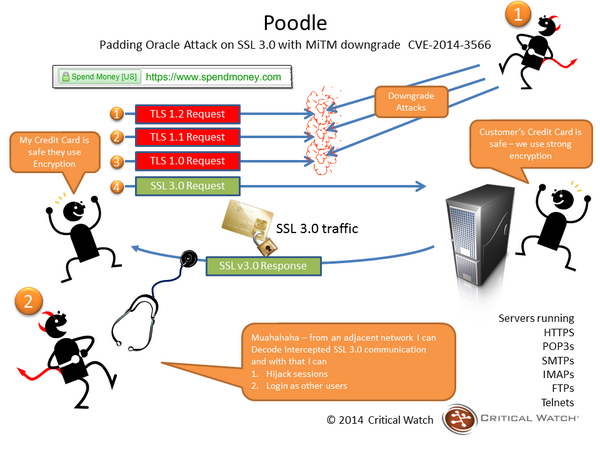
\includegraphics[scale=0.7]{pics/poodle.png}
		\caption{Принцип работы атаки POODLE} 
		\label{pic:pic_name}
	\end{center}
\end{figure}


\subsubsection{HeartBleed}

\textbf{HeartBleed} (CVE-2014-0160) - ошибка, заключающаяся в переполнении буфера в OpenSSL. Позволяет несанкционированно читать память на сервере или клиенте, в том числе и для извлечения закрытого ключа сервера. Информация об уязвимости была опубликована в апреле 2014 года, ошибка существовала с конца 2011 года. SSLv3 на тот момент использовали многие сайты, в том числе банки, платёжные системы, VPN-провайдеры, сервисы почты Yandex и Yahoo.

Подробная информация об уязвимости размещена на специальном сайте, посвящённом ей.\footnote{\url{http://heartbleed.com/}}. Между тем, забавно, но при подключении по HTTPS к этой странице, выясняется, что соединение не защищено и появляется ошибка ERR\_CERT\_COMMON\_NAME\_INVALID.

Название HeartBleed происходит от названия реализации TLS/DTLS расширения Heartbeat, в котором была найдена уязвимость. В результате эксплойта можно добиться утечки памяти как с сервера на клиент, так и с клиента на сервер. При этом никаких следов атака не оставляет, и, учитывая долгое время поддержания подключения, невозможно установить, как много и какая информация стала доступна злоумышленнику.

Схематично атаку можно изобразить следующим образом следующим образом:

\begin{figure}[H]
	\begin{center}
		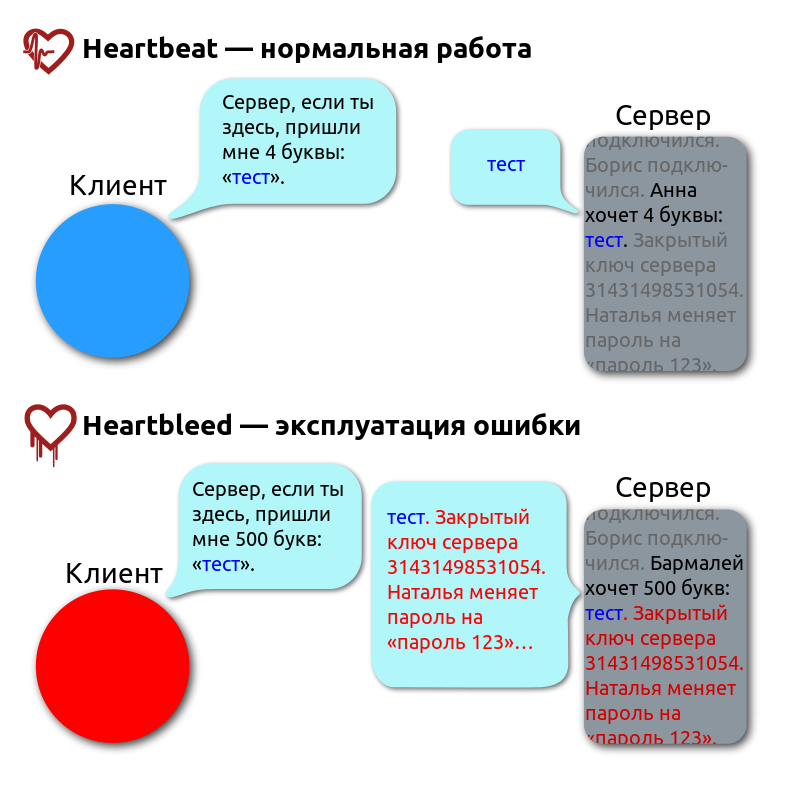
\includegraphics[scale=0.4]{pics/heartbleed.png}
		\caption{Принцип работы атаки Heartbleed} 
		\label{pic:pic_name}
	\end{center}
\end{figure}

\newpage

\section{Практическое задание}

Выбрать со стартовой страницы SSL Server Test один домен из списка Recent Best и один домен из списка Recent Worst – изучить отчеты, интерпретировать результаты в разделе Summary. Выбрать для анализа интернет-домен защищенный SSL-шифрованием (старайтесь выбрать что-то достаточно известное, но не слишком очевидное), проделать следующие шаги:

\subsection{Recent Best}

\subsubsection{Интерпретировать результаты в разделе Summary}

\begin{figure}[H]
	\begin{center}
		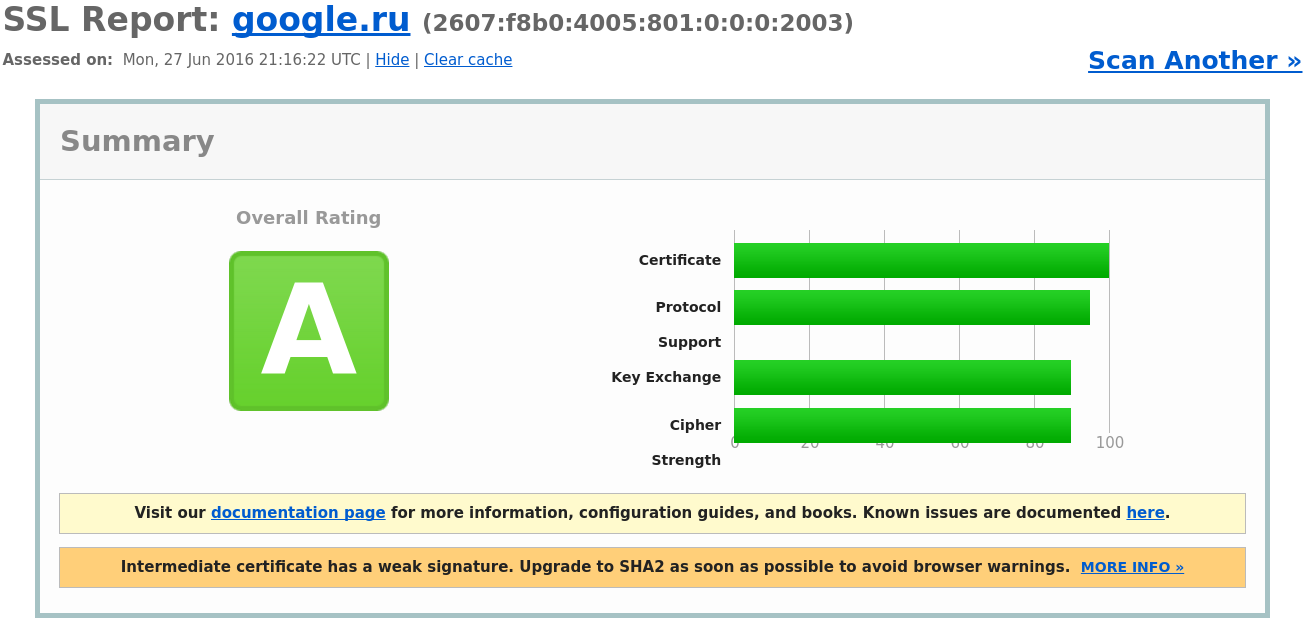
\includegraphics[scale=0.4]{pics/google.ru.png}
		\caption{Recent best: google.ru (google.com/google.at/...)} 
		\label{pic:pic_name}
	\end{center}
\end{figure}

Google.com выбран, как наиболее известный домен, одна из вариаций которого (google.at) была обнаружена в recent best. Однако это не наилучший результат (A). Вот пример лучшего результата (A+):

\begin{figure}[H]
	\begin{center}
		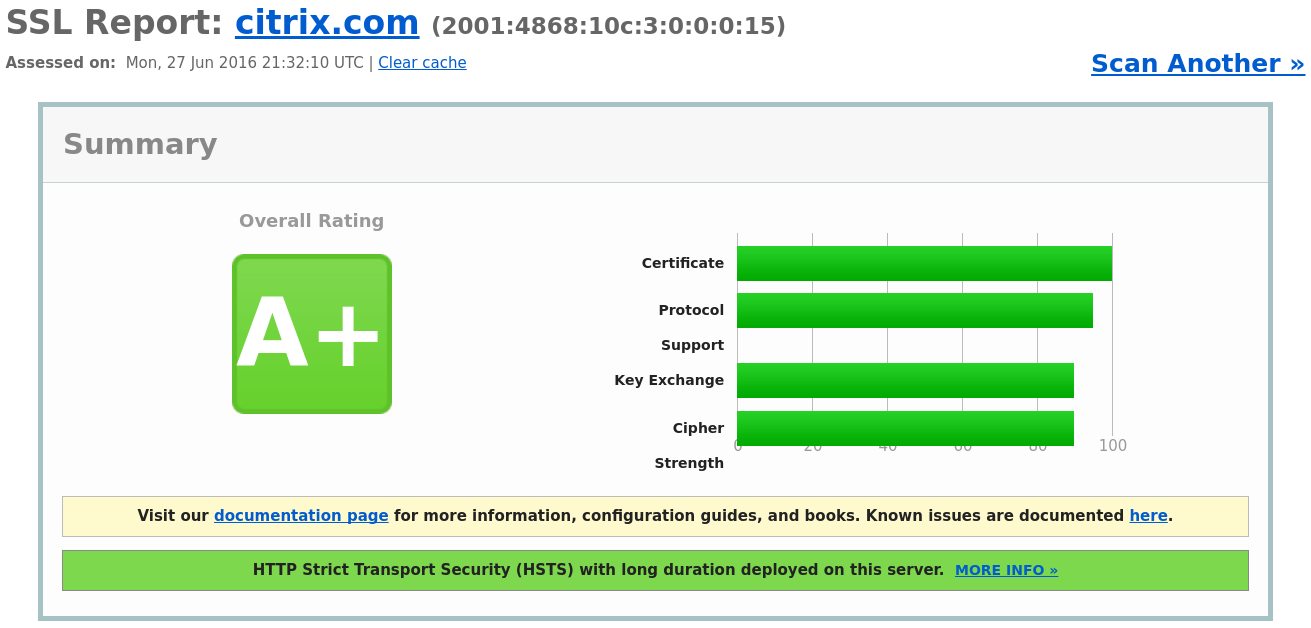
\includegraphics[scale=0.35]{pics/citrix.png}
		\caption{Recent best A+: citrix.com} 
		\label{pic:pic_name}
	\end{center}
\end{figure}

Интересно, что сигнатура одинаковая - RSA. Однако строчка описывается по-разному для сайтов. Для citrix.com:

\begin{verbatim}
Signature algorithm	SHA1withRSA   Weak, but no impact on root certificate
\end{verbatim}

Для сайта google.ru::

\begin{verbatim}
Signature algorithm	SHA1withRSA   WEAK
\end{verbatim}

Однако для citrix.com есть пометка "DigiCert Global Root CA   In trust store ". Т.е. доверие Root CA перевешивает недостаточно стойкий, по мнению SSLLabs, алгоритм подписи.

\subsubsection{Расшифровать все аббревиатуры шифров в разделе Configuration}

\begin{lstlisting}[numbers=none, keywords={}]
Protocols
TLS 1.2	Yes
TLS 1.1	Yes
TLS 1.0	Yes
SSL 3	No
SSL 2	No
\end{lstlisting}

Таким образом, поддерживает все современные надёжные протоколы и не поддерживает скомпрометированные SSLv3 и SSLv2.

\begin{lstlisting}[numbers=none, keywords={}]
Cipher Suites (SSL 3+ suites in server-preferred order; deprecated and SSL 2 suites at the end)
TLS_ECDHE_RSA_WITH_AES_128_GCM_SHA256 (0xc02f)   ECDH secp256r1 (eq. 3072 bits RSA)   FS	128
OLD_TLS_ECDHE_RSA_WITH_CHACHA20_POLY1305_SHA256 (0xcc13)   ECDH secp256r1 (eq. 3072 bits RSA)   FS	256P
TLS_ECDHE_RSA_WITH_CHACHA20_POLY1305_SHA256 (0xcca8)   ECDH secp256r1 (eq. 3072 bits RSA)   FS	256P
TLS_ECDHE_RSA_WITH_AES_128_CBC_SHA (0xc013)   ECDH secp256r1 (eq. 3072 bits RSA)   FS	128
TLS_RSA_WITH_AES_128_GCM_SHA256 (0x9c)	128
TLS_RSA_WITH_AES_128_CBC_SHA (0x2f)	128
TLS_RSA_WITH_AES_128_CBC_SHA256 (0x3c)	128
TLS_RSA_WITH_3DES_EDE_CBC_SHA (0xa)	112
TLS_ECDHE_RSA_WITH_AES_256_GCM_SHA384 (0xc030)   ECDH secp256r1 (eq. 3072 bits RSA)   FS	256
TLS_ECDHE_RSA_WITH_AES_128_CBC_SHA256 (0xc027)   ECDH secp256r1 (eq. 3072 bits RSA)   FS	128
TLS_ECDHE_RSA_WITH_AES_256_CBC_SHA (0xc014)   ECDH secp256r1 (eq. 3072 bits RSA)   FS	256
TLS_ECDHE_RSA_WITH_AES_256_CBC_SHA384 (0xc028)   ECDH secp256r1 (eq. 3072 bits RSA)   FS	256
TLS_RSA_WITH_AES_256_GCM_SHA384 (0x9d)	256
TLS_RSA_WITH_AES_256_CBC_SHA (0x35)	256
TLS_RSA_WITH_AES_256_CBC_SHA256 (0x3d)	256
(P) This server prefers ChaCha20 suites with clients that don't have AES-NI (e.g., Android devices)	

\end{lstlisting}

Аббревиатуры:

\begin{verbatim}
TLS - transport layer security
ECDHE - elliptic curve Diffie-Hellman ephemeral
RSA - Rivest, Shamir, Adelman
AES - American encryption standard
GCM SHA-256 - secure hash algorithm (256-bits) with Galois/counter mode
ChaCha - stream cipher
Poly1305 - cryptographic message authentication code
CBC - chipher block chaining
\end{verbatim}



\subsubsection{Прокомментировать большинство позиций в разделе Protocol Details}

\begin{figure}[H]
	\begin{center}
		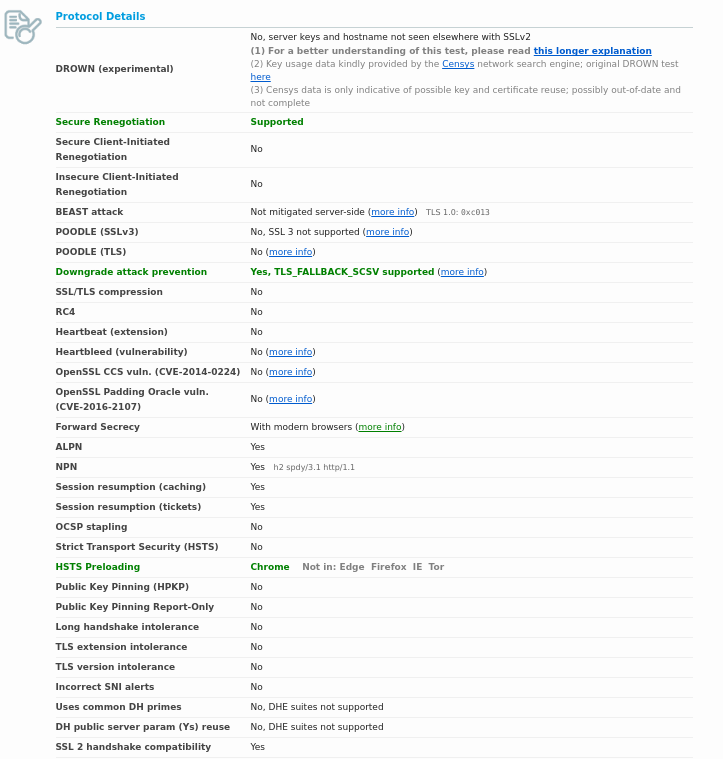
\includegraphics[scale=0.6]{pics/google_protocol_details.png}
		\caption{Protocol details} 
		\label{pic:pic_name}
	\end{center}
\end{figure}

Сервис не поддерживает опасные протоколы, скомпрометированный потоковый шифр RC4, опасную версию OpenSSL, тем самым исключая распространённые атаки: DROWN, BEAST, POODLE, Heartbleed. Поддерживает безопасное повторное установление соединения, поддерживает ALPN, закрепление открытого ключа, HSTS предзагрузку, OSCP stapling. 

\subsubsection{Сделать итоговый вывод о реализации SSL на заданном домене}

Данный домен в большой степени удовлетворяет приведённым в начале работы современным критериям безопасности использования SSL/TLS. Он использует большинство современных и продвинутых технологий, при этом исключает взаимодействие посредством скомпрометированных протоколов.

\subsection{Recent Worst}

\subsubsection{Интерпретировать результаты в разделе Summary}

\begin{figure}[H]
	\begin{center}
		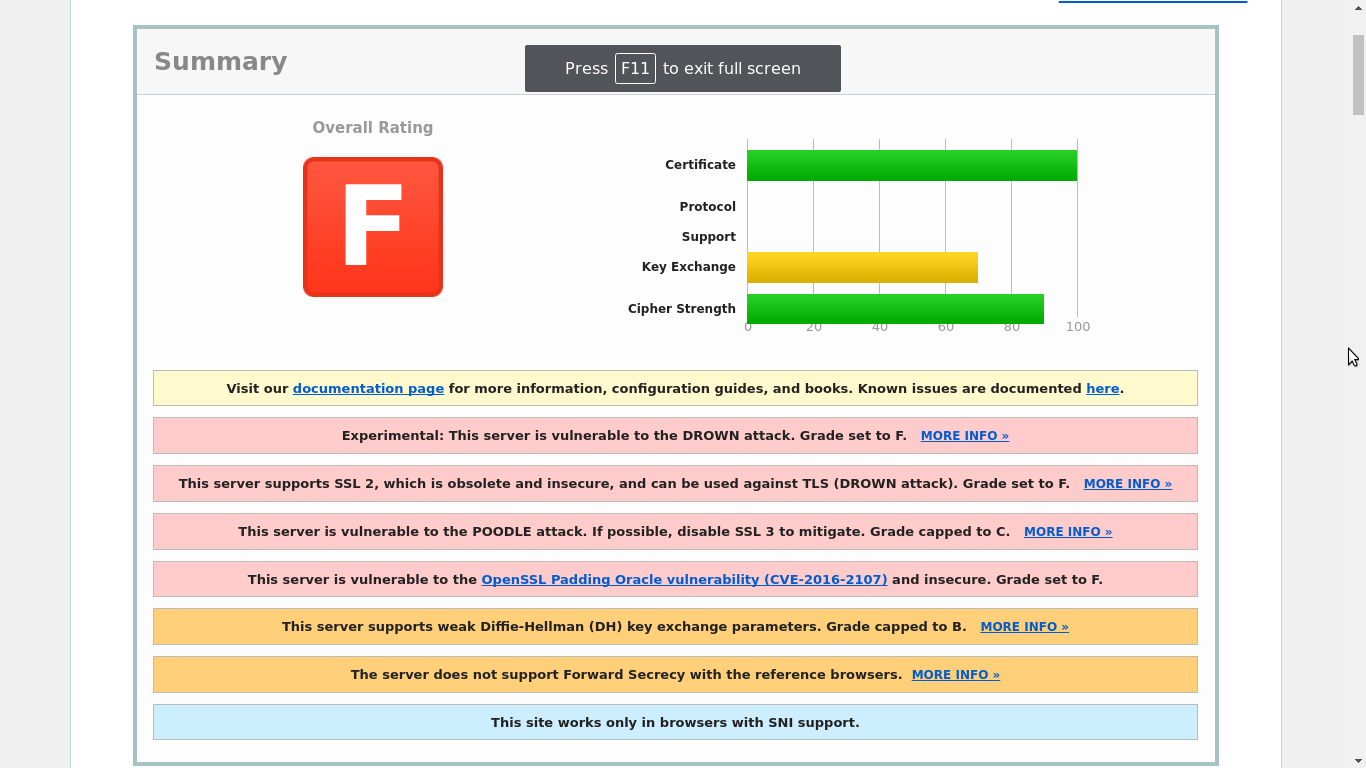
\includegraphics[scale=0.4]{pics/worst.myplan.moreactive.com.png}
		\caption{Recent worst: myplan.moreactive.com} 
		\label{pic:pic_name}
	\end{center}
\end{figure}

\subsubsection{Расшифровать все аббревиатуры шифров в разделе Configuration}

\begin{lstlisting}[numbers=none, keywords=none]

Protocols
TLS 1.2	Yes
TLS 1.1	Yes
TLS 1.0	Yes
SSL 3 2   INSECURE	Yes
SSL 2 2   INSECURE	Yes
(2) This site requires support for virtual secure hosting (SNI), but SSL 2 and SSL 3 do not support this feature.


Cipher Suites (SSL 3+ suites in server-preferred order; deprecated and SSL 2 suites at the end)
TLS_DHE_RSA_WITH_AES_256_GCM_SHA384 (0x9f)   DH 1024 bits   FS   WEAK	256
TLS_DHE_RSA_WITH_AES_256_CBC_SHA256 (0x6b)   DH 1024 bits   FS   WEAK	256
TLS_DHE_RSA_WITH_AES_256_CBC_SHA (0x39)   DH 1024 bits   FS   WEAK	256
TLS_DHE_RSA_WITH_CAMELLIA_256_CBC_SHA (0x88)   DH 1024 bits   FS   WEAK	256
TLS_RSA_WITH_AES_256_GCM_SHA384 (0x9d)	256
TLS_RSA_WITH_AES_256_CBC_SHA256 (0x3d)	256
TLS_RSA_WITH_AES_256_CBC_SHA (0x35)	256
TLS_RSA_WITH_CAMELLIA_256_CBC_SHA (0x84)	256
TLS_DHE_RSA_WITH_AES_128_GCM_SHA256 (0x9e)   DH 1024 bits   FS   WEAK	128
TLS_DHE_RSA_WITH_AES_128_CBC_SHA256 (0x67)   DH 1024 bits   FS   WEAK	128
TLS_DHE_RSA_WITH_AES_128_CBC_SHA (0x33)   DH 1024 bits   FS   WEAK	128
TLS_DHE_RSA_WITH_CAMELLIA_128_CBC_SHA (0x45)   DH 1024 bits   FS   WEAK	128
TLS_DHE_RSA_WITH_3DES_EDE_CBC_SHA (0x16)   DH 1024 bits   FS   WEAK	112
TLS_RSA_WITH_AES_128_GCM_SHA256 (0x9c)	128
TLS_RSA_WITH_AES_128_CBC_SHA256 (0x3c)	128
TLS_RSA_WITH_AES_128_CBC_SHA (0x2f)	128
TLS_RSA_WITH_CAMELLIA_128_CBC_SHA (0x41)	128
TLS_RSA_WITH_3DES_EDE_CBC_SHA (0xa)	112

\end{lstlisting}

Этот сервис поддерживает использование скомпрометированных протоколов SSLv3 и SSLv2.

Также видим, что для большинства протоколов используется пометка WEAK.

Аббревиатуры:

\begin{verbatim}
TLS - transport layer security
DHE - Diffie-Hellman ephemeral
RSA - Rivest, Shamir, Adelman
AES - American encryption standard
Camelia - symmetric key block cipher
GCM SHA-384 - secure hash algorithm (384-bits) with Galois/counter mode
CBC - chipher block chaining
3DES - triple data encryption standard
EDE - mode of 3DES (encrypt - decrypt - encrypypt)
\end{verbatim}

\subsubsection{Прокомментировать большинство позиций в разделе Protocol Details}

\begin{figure}[H]
	\begin{center}
		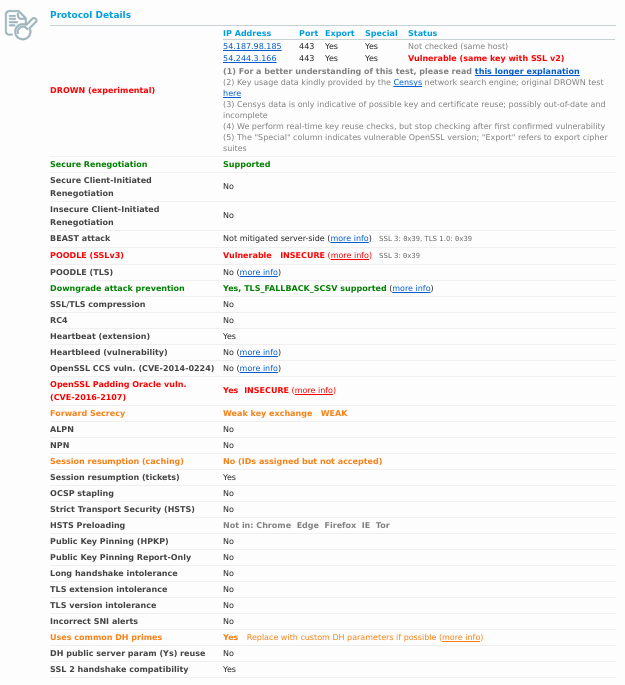
\includegraphics[scale=0.7]{pics/moreactive.com_protocol_details.png}
		\caption{Protocol details for myplan.moreactive.com} 
		\label{pic:pic_name}
	\end{center}
\end{figure}

Данный сервер поддержен DROWN-атаке, потому что он поддерживает SSLv2 и закрытый ключ используется другим сервером, поддерживающим SSLv2. Схематично она изображена ниже.

\begin{figure}[H]
	\begin{center}
		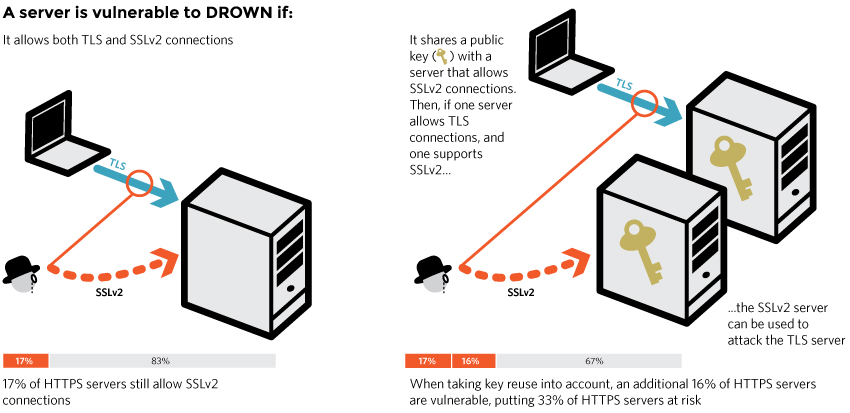
\includegraphics[scale=0.4]{pics/drown_diag.jpg}
		\caption{Схема DROWN-атаки} 
		\label{pic:pic_name}
	\end{center}
\end{figure}

Так как сервер поддерживает SSLv3, он подвержен атаке POODLE, а также ещё одной подобной атаке - OpenSSL Padding Oracle vuln.

Сервер поддерживает слабый Forward Security, не поддерживает возобновление сеанса, использует распространённые простые числа для алгоритма Диффи-Хеллмана. 

Остальные настройки в порядке. Сервис не подвержен атаке POODLE по TLS, BEAST-атаке, а также Heartbleed. Поддерживает безопасное повтороное установление соединения. Поддерживает Downgrade attack prevention. Продвинутых возможностей, таких как HSTS preloading, OCSP stapling не поддерживает.

\subsubsection{Сделать итоговый вывод о реализации SSL на заданном домене}

Таким образом, домен имеет довольно слабую защиту от взлома SSL/TLS. Он подвержен атакам на протоколы SSLv2 и SSLv3 в силу их использования. Алгоритмы, используемые в настройках домена, в настоящее время считаются слабыми и устаревшими. В результате, имеем плохо защищённый домен, SSL/TLS на котором можно взломать. 

\section{Выводы}

В настоящее время безопасность передачи данных по защищённым протоколам, используемым асимметричные алгоритмы, является крайне важной в силу их постоянного использования и совершенствования средств и методик проведения атак и нахождения уязвимостей. Решающую роль в данном случае имеет человеческий фактор - своевременное реагирование на инцеденты, регулярное обновление ПО, отвечающего за безопасность и, немаловажно, правильная и грамотная его настройка. Существуют рекомендации по использованию SSL/TLS, которые регулярно обновляются и совершенствуются в соответствии с тенденциями мира информационной безопасности. Если следовать этим рекомендациям, шанс на взлом соединения и утечку конфиденциальных данных практически отсутствует.

Несмотря на открытую информацию о необходимой конфигурации систем с SSL/TLS, немалое количество доменов всё же имеют настройки, позволяющие проводить атаки на используемые протоколы. Используются устаревшие и скомпрометированные протоколы и шифры, несмотря на очевидность недопустимости их использования для обеспечения безопасности. Главной причиной, как уже было указано выше, является человеческий фактор.

\end{document}